\chapter{Theoretical Overview}

\index{čeština v rejstříku}

\section{Overview of Neural Networks}
\label{sec:overview-neural-networks}

\textcolor{pink}{Do neural networks need feature selection?
Does overparameterization reduce need for sparsity?
What is the trade-off between predictive accuracy and interpretability?
How does correlated input affect selection stability?
Can feature selection harm representation learning?}

Neural networks are one of the most popular algorithms of machine learning. Their were inspired by the structure and function of biological neurons, which are the fundamental units of nervous tissue. To distinguish them from their biological counterpart, sometimes the term \textit{Artificial neural networks (ANNs)} is used. 

Neural network can be viewed as a composition of affine transformations and non-linear activation functions, which allows them to serve as universal approximators. This property is established in many theorems; several of which are mentioned by Goodfellow in \cite{goodfellow2016}. Their ability to capture complex patterns makes them widely applicable in areas such as computer vision, natural language processing, and predictive modeling. A detailed treatment of neural network applications and methodologies can be found in the comprehensive review by Abiodun et al. \cite{abiodun2019}.

 
\textcolor{orange}{ ? including one relevant theorem for deep networks by Kidger and Lyons: }

\subsection{Network architectures}
\label{sec:network-architectures}
\textbf{Neuron} \\
These networks are called \textit{neural} because their structure is loosely inspired by neuroscience. Basic computational unit of a neural network is the \textit{(artificial )neuron}. Formally, a neuron is a function 
\[
f_{\mathbf{w},b}: \mathbb{R}^n \to \mathbb{R}, \quad \mathbf{x} \mapsto f_{\mathbf{w},b}(\mathbf{x}) = f\Big(\mathbf{w}^\top \mathbf{x} + b\Big) = f\Big(\sum_{i=1}^{n} w_i x_i + b\Big),
\]
where $\mathbf{x} = (x_1, \dots, x_n)^\top \in \mathbb{R}^n$ is the input vector, $\mathbf{w} = (w_1, \dots, w_n)^\top \in \mathbb{R}^n$ is the vector of trainable weights, $b \in \mathbb{R}$ is the bias term, and $f: \mathbb{R} \to \mathbb{R}$ is a nonlinear activation function. The structure of a single neuron is illustrated in Figure~\ref{fig:neuron}.


\textcolor{pink}{A Little Diagram}
\begin{figure}[ht]
    \centering
    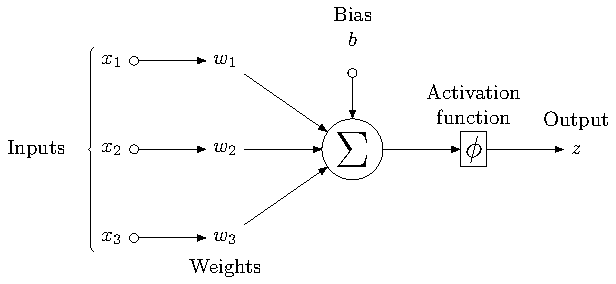
\includegraphics[width=1\textwidth]{figures/tikz3.pdf}
    \caption{Schematic of a single artificial neuron}
    \label{fig:neuron}
\end{figure}


\textbf{Architecture of the network} \\
The architecture of a neural network describes how neurons and layers are organized, connected, and how they transform information. A network typically consists of an input layer that receives data, hidden layers that perform computations, and an output layer that produces predictions (see Figure \ref{fig:neural-network}).



\begin{figure}[ht]
    \centering
    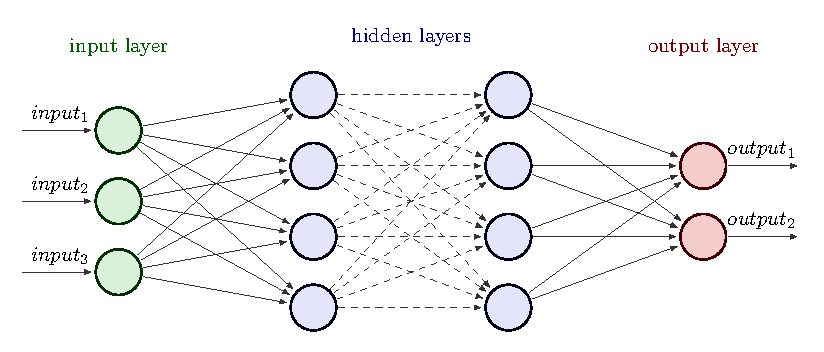
\includegraphics[width=1\textwidth]{figures/tikz1.pdf}
    \caption{Scheme of the Neural Network}
    \label{fig:neural-network}
\end{figure}



Neurons in hidden layer work the same way as a perceptrons, except that instead of receiving the input vector, they take the outputs of neurons from the previous layer. Because of this similarity those networks are also called \textit{multilayer perceptron}. When the information flows strictly in one direction - from input layer to output layer, we refer to the architecture as \textit{feedforward network}. On the contrary, it is common for all neurons in the hidden layers to share the same activation function, though this is not required; the choice of activation functions will be discussed in the \textcolor{green}{Subsection XXX}. Likewise, the hidden layers do not need to have the same number of neurons, as it is illustrated in Figure~\ref{fig:convolutional-neural-network}.


The flow of signals in networks does not have to be strictly one-directional. In some cases, we want to process a sequence of inputs with respect to their order. For such sequential data \textit{recurrent networks} are used, in which neurons are able to store information from earlier signal passes and take it into account during future activations (see Figure~\ref{fig:reccurent-neural-network}).. It is implemented by creating loops between neurons to allow information to persist across time steps. These properties are essential for tasks such as time series modeling or human speech recognition.

\textcolor{pink}{TODO: Plot the graph in latex}

\begin{figure}[ht]
    \centering
    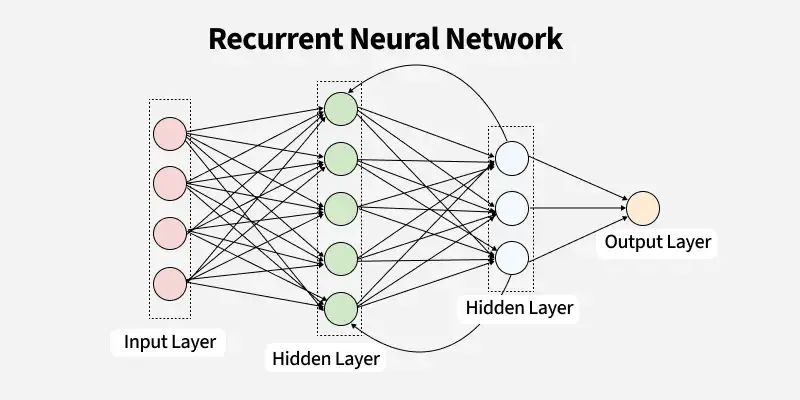
\includegraphics[width=1\textwidth]{figures/recurrent_neural_network.png}
    \caption{Scheme of the Recurrent Neural Network}
    \label{fig:reccurent-neural-network}
\end{figure}

It is also not necessary for neural networks to use a fully connected architecture. A partially connected structure is used in \textit{convolutional networks} (see Figure~\ref{fig:convolutional-neural-network}), mainly applied to image and character recognition. Their idea is to alternate \textit{convolutional and pooling layers}: the input is broken into small patches, which are processed through repeated layers. Early layers detect simple patterns like edges, while later ones combine them into more complex shapes. Because the connections are sparse, training is faster, and with the right design, convolutional networks can achieve very strong performance in image recognition \cite{lecun2015}.

% DEEP CONVOLUTIONAL NEURAL NETWORK
\begin{figure}[ht]
\centering
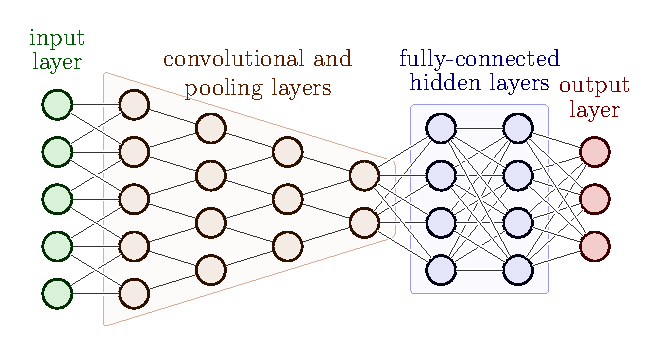
\includegraphics[width=0.8\textwidth]{figures/tikz2.pdf}
\caption{Scheme of the Convolutional Neural Network}
\label{fig:convolutional-neural-network}
\end{figure}



The architecture of a network is therefore determined by the number of hidden layers, their width (the number of neurons in each layer), the way the neurons are connected, and the manner in which the signal flows.

\textbf{Notation} \textcolor{orange}{introduce notation}

\subsection{Notation}
\label{sec:notation}
The activation of the \(j\)-th neuron in the \(i\)-th layer is computed as a weighted sum of the inputs from the previous layer plus a bias, passed through an activation function:
\[
a_j^{(i)} = 
\sigma\Big( \sum_{k=1}^{n} w_{j,k}^{(i)} a_k^{(i-1)} + b_j^{(i)} \Big) = \sigma\Big( \mathbf{w}_j^{(i)} \cdot \mathbf{a}^{(i-1)} + b_j^{(i)} \Big),
\]
where \(\mathbf{w}_j^{(i)} = (w_{j,1}^{(i)}, w_{j,2}^{(i)}, \dots, w_{j,n}^{(i)})\) is the weight vector of the \(j\)-th neuron,\\ \(\mathbf{a}^{(i-1)} = (a_1^{(i-1)}, a_2^{(i-1)}, \dots, a_n^{(i-1)})^\top\) is the input vector from the previous layer, and \(b_j^{(i)}\) is the bias term in the \(i\)-th layer and in the \(j\)-th neuron.


For the entire layer of \(m\) neurons, the activations can be written in vector form:
\[
\begin{pmatrix}
a_1^{(i)}\\
a_2^{(i)}\\
\vdots\\
a_m^{(i)}
\end{pmatrix}
=
\sigma\left(
\begin{pmatrix}
w_{1,1}^{(i)} & w_{1,2}^{(i)} & \dots & w_{1,n}^{(i)} \\
w_{2,1}^{(i)} & w_{2,2}^{(i)} & \dots & w_{2,n}^{(i)} \\
\vdots & \vdots & \ddots & \vdots \\
w_{m,1}^{(i)} & w_{m,2}^{(i)} & \dots & w_{m,n}^{(i)}
\end{pmatrix}
\begin{pmatrix}
a_1^{(i-1)}\\
a_2^{(i-1)}\\
\vdots\\
a_n^{(i-1)}
\end{pmatrix}
+
\begin{pmatrix}
b_1^{(i)}\\
b_2^{(i)}\\
\vdots\\
b_m^{(i)}
\end{pmatrix}
\right).
\]

In compact vector-matrix notation, this can be written as:
\[
\mathbf{a}^{(i)} = \sigma\Big( \mathbf{W}^{(i)} \mathbf{a}^{(i-1)} + \mathbf{b}^{(i)} \Big),
\]
where \(\mathbf{W}^{(i)}\) is the weight matrix connecting layer \(i-1\) to layer \(i\), \(\mathbf{a}^{(i-1)}\) is the input vector, \(\mathbf{b}^{(i)}\) is the bias vector, and \(\mathbf{a}^{(i)}\) is the vector of activations in layer \(i\).


This illustrates that the operation of a neural network layer can be equivalently expressed in element-wise form, summation form, or vector-matrix form.

\subsection{Brief History of Neural Networks}
\label{sec:brief-notation}
\textbf{Origins:} In 1949, Canadian psychologist Donald Hebb proposed that the connections (synapeses) between neurons strengthen when they are activated together \cite{hebb1949}. This is often summarized by the phrase attributed to him: “neurons that fire together, wire together”. So called \textit{Hebbian theory} provided a foundational idea, that networks could learn from experience.

\textbf{Early models:} A year later, the \textit{Perceptron}, introduced by Frank Rosenblatt \cite{rosenblatt1958}, was the first type of neural network designed to learn from examples. It combined the concept of a computational neuron with a learning algorithm that automatically adjusted its weights to separate inputs into classes using a linear decision boundary. The Perceptron was a single-layer neural network that applied a Heaviside (binary step) activation function to an affine combination of the inputs, producing a binary output. As a linear classifier, its decision boundary is a hyperplane in the input space, which means it can only correctly classify linearly separable data. Though groundbreaking, this linearity limited its ability to solve more complex classification problems. \textcolor{pink}{Sidenote: Watching movies and documentaries is a valid research and you can cite them as well :) If you're lucky, some of these people even spoke about their research on TV, in public seminars, talks and such. I'd scout youtube for some which were uploaded publicly. }

\textbf{Setback:} The work of Minsky and Papert in \cite{minsky1969} demonstrated that single-layer linear networks could not solve problems such as the XOR function, which led to a temporary decline in research of neural networks \cite{lecture1_2017}. \textcolor{orange}{ Reference to paragraph in this thesis discussing limitations of perceptron capturing logic of XOR function in this thesis (maybe in similar way as it is showed by Goodfellow)}
\textcolor{pink}{TODO: Plot the graph in latex}

\textbf{Revival:} Neural networks regained attention with the development of multi-layer networks trained using backpropagation \cite{rumelhart1986}, \textcolor{green}{which will be discussed in Section X}.. This allowed networks to learn more complex patterns and revived research in deep learning.

\textbf{Specialised networks:} In the 1990s researchers introduced specialized architectures for different types of data. The development of \textit{convolutional neural networks}, as presented by LeCun, Bottou, Bengio, and Haffner in \cite{lecun1998}, for image processing, together with the use of \textit{recurrent neural networks} for sequential data, enabled neural networks to tackle a wider variety of problems. This led to strong improvements in vision, speech, and language applications \cite{lecun2015}.


\textbf{Developments up to 2026:} Breakthroughs such as AlexNet \cite{krizhevsky2012} and the \textit{transformer} architecture - built on the attention mechanism \cite{vaswani2017} - accelerated progress in image recognition and natural language processing. \textit{The attention mechanism} allows a neural network to focus on the most relevant parts of the input when making a prediction. Instead of treating all inputs equally, the model computes attention weights that measure how important each element (for example, each word in a sentence) is for the current step. This makes the model better at capturing long-range relationships and understanding context efficiently.

\subsection{Activation functions in the hidden Layer}
\label{sec:activation-functions-hidden-layer}
Activation function introduce non-linearity into model to learn complex data patterns. Without it, even a deep neural network would behave like a simple linear regression model.
\textcolor{orange}{aproximation of general functions by neural networks}

The earliest neural networks relied on smooth, bounded activation functions such as the \textit{sigmoid} and \textit{hyperbolic tangent (tanh)}. The sigmoid function:

\[
\phi(x) = \frac{1}{1 + e^{-x}}
\]

compresses the input to the interval \((0,1)\) and has a simple derivative:  

\[
\phi'(x) = \phi(x)\bigl(1 - \phi(x)\bigr),
\]

which makes effective computation during \textit{backpropagation algorithm}, which is discussed in \textcolor{green}{Section xx}

However, for very large positive or negative inputs, the sigmoid function approaches its asymptotes, causing its derivative to become very small. This can lead to extremely small gradients, contributing to the well-known \textit{vanishing gradient problem} \cite{goodfellow2016}. A similar issue arises with the $\tanh$ function 

\[
\phi(x) = \tanh(x) = \frac{1 + e^{-2x}}{1 - e^{-2x}}.
\]


In contrast, the \textit{exploding gradient problem} occurs when gradients grow exponentially during \textit{backpropagation}, leading to unstable learning \cite{goodfellow2016}. Both gradient-related problems and the backpropagation algorithm \textcolor{green}{will be discussed in detail in Subsection~XX}.


 A major breakthrough came with the introduction of the \textit{ReLU (Rectified Linear Unit)} defined as

\[
\phi(x) = \max(\{0, x\}).
\]

ReLU is computationally more efficient than sigmoidal functions, avoids saturation for positive inputs, and converges faster in deep architectures \cite{aggarwal2018}. 

Main problem with ReLU as activation function is that in learning process it is prone to creating so-called \textit{dead neurons}. This is a phenomenon, when its pre-activation value $w^Tx + b$ consistently falls into the non-positive region, causing its output to remain zero for given inputs during a training process. Since their gradient is always zero, their weights stop updating and they no longer contribute to learning.

To cope with such issue, several variants have been proposed. \textit{Leaky ReLU} uses small slope for negative inputs $\phi(x) = \max(\alpha x, x)$, where $\alpha$ is a small positive constant (typically 0.01), which prevents complete inactivity. Another widely used alternative is the \textit{Gaussian Error Linear Unit (GELU)}. Hendrycks and Gimpel in \cite{hendrycks2016} showed that its smooth, probabilistic, Gaussian-based formulation improves performance across a variety of tasks. GELU has become a standard choice in transformer-based architectures, including models such as 
\textit{Generative Pre-trained Transformer (GPT)} \cite{radford2019} and \textit{Bidirectional Encoder Representations from Transformers (BERT)} \cite{devlin2018}.

\subsection{Activation Functions in Output Layer}
\label{sec:activation-functions-ouput-layer}

The choice of activation function in the output layer of a neural network depends on the type of task and the desired output representation. For regression tasks, where the network predicts continous values, the \textit{identity function} $\phi(x) = x$ is commonly used. 

For binary classification, the sigmoid function \textcolor{green}{Section XX} is frequently used. Its output lies in the interval $(0,1)$, which can be interpreted as the probability of belonging to a positive class. Its differentiability enables efficient gradient-based learning.

For multiclass classification, the \textit{softmax} function is commonly used. Given an input vector 
\(\mathbf{x} = (x_1, x_2, \dots, x_k)^\top \in \mathbb{R}^k\), softmax maps it to a probability distribution over \(k\) classes:

\[
\mathrm{softmax}(x_i) = \frac{e^{x_i}}{\sum_{j=1}^{k} e^{x_j}}, \quad i = 1,2, \dots, k.
\]

This ensures that \(\mathrm{softmax}(x_i) > 0\) $\forall$ \(i\) and \(\sum_{i=1}^{k} \mathrm{softmax}(x_i) = 1\), allowing the outputs to be interpreted as class probabilities. For this transformation to work, the last hidden layer must have the same number of neurons as the output layer, and its outputs are fed directly into the softmax, with no additional weights.

\subsection{Loss Functions}
\label{sec:loss-functions}
Loss function quantifies the difference between a neural network's prediction $\hat{y}$ and target value $y$. It can be used to both evaluate performance of the model, and for guidence in gradient-based learning, as it will be illustrated in the following subsection. Our goal is to minimize the prediction error by optimizing the loss function.

The choice of loss function depends on the type of task. For regression tasks, the \textit{mean squared error} is commonly used:

\[
    \mathcal{L} = \text{MSE} = \frac{1}{n}\sum_{i=1}^{n}{\left(y_i - \hat{y}_i\right)^2}
\]

For binary classification, the \textit{binary cross-entropy} loss is used, which is the the negative log-likelihood of Bernoulli distribution:

\[
\mathcal{L} = - \frac{1}{n} \sum_{i=1}^{n} \Big[ y_i \log \hat{y}_i + (1 - y_i) \log (1 - \hat{y}_i) \Big],
\]

where \(\hat{y}_i\) represents the predicted probability of the positive class.

For multiclass classification, the \textit{categorical cross-entropy loss} is used in combination with the softmax activation:

\[
\mathcal{L} = - \frac{1}{n} \sum_{i=1}^{n} \sum_{k=1}^{k} y_{i,k} \log \hat{y}_{i,k},
\]

where 

\[
y_{i,k} = 
\begin{cases} 
1 & \text{if sample $i$ belongs to class $k$,} \\
0 & \text{otherwise,} 
\end{cases}
\]

and \(\hat{y}_{i,k}\) is the predicted probability for class $k$  of sample $i$ .

\subsection{Gradient Descent}
\label{sec:gradient-descent}
Gradient descent is an optimization algorithm used to train neural networks by minimizing loss function. Its main idea is iteratively adjusting the parameters of the model in the the direction that reduces loss the most. Formally, for a set of parameters $\boldsymbol{\theta}$ and a differentiable loss function $\mathcal{L}(\boldsymbol{\theta})$, the update rule naturally is:


\[
\boldsymbol{\theta}_{t+1} = \boldsymbol{\theta}_t - \eta \, \nabla_{\boldsymbol{\theta}} \mathcal{L}(\boldsymbol{\boldsymbol{\theta}}_t),
\]


where $\eta \in \mathbb{R}_{>0}$ is a hyperparameter called \textit{learning rate}, which controls step size, and $\nabla_{\boldsymbol{\theta}}\mathcal{L}(\boldsymbol{\theta})$ is the gradient of loss function with respect to all parameters at iteration $t$.

Under conditions such as convexity and Lipshitz-continuity of gradients, convergence to the global minimum is guaranteed. However, these conditions are rarely satisfied in practice and thus the algorithm may converge to a local minimum, diverge or oscillate.



There are multiple ways in which the parameters can be updated at each step, depending on the choice of \textit{batch} - subset of training data used to estimate the gradient. In \textit{batch gradient descent}, the gradient is computed over the entire dataset:

\[
\boldsymbol{\theta}_{t+1} = \boldsymbol{\theta}_t - \eta \, \frac{1}{n} \sum_{i=1}^{n} \nabla_{\boldsymbol{\theta}} \mathcal{L}(\boldsymbol{\theta}_t, y_i),
\]

where \(n\) is the total number of training samples and \(\mathcal{L}(\boldsymbol{\theta}_t, y_i)\) is the loss for a single sample. This provides an accurate update but can be computationally expensive for large datasets.


In \textit{stochastic gradient descent}, the parameters are updated using a single randomly selected training sample per iteration:

\[
\boldsymbol{\theta_{t+1}} = \boldsymbol{\theta_t} - \eta \, \nabla_{\boldsymbol{\theta}} \mathcal{L}(\boldsymbol{\theta_t}, y_i),
\]

which introduces stochasticity, potentially helping the optimizer escape shallow local minima.

\textit{Mini-batch gradient descent} updates the parameters using a small subset of size $B$, where $B \in \mathbb{N}$ and $1 < B < n$:


\[
\boldsymbol{\theta}_{t+1} = \boldsymbol{\theta}_t - \eta \, \frac{1}{B} \sum_{i \in \text{mini-batch}} \nabla_{\boldsymbol{\theta}} \mathcal{L}(\boldsymbol{\theta}_t, y_i),
\]


This approach is the most commonly used in practice, because of its computational efficiency and smoother convergence \cite{gfg2025}.

It is important to mention the \textit{backpropgation algorithm}, which is used for effective computation of gradient of a loss function. It applies the chain rule of calculus to propagate from the output layer backward through the network and iteratively compute weights and biases. This reduces the overall computational complexity from exponential to linear with regard in the number of layers \cite{goodfellow2016}.

For effective learning, it is crucial to choose appropriate learning rate. It controls magnitude of each step in a gradient-descent. A small learning rate can cause slow convergence. Conversely, a too large learning rate can cause divergence, or oscillatory behavior. Thus, selecting a fixed learning rate can cause instability or excessively slow convergence during training. Several modifications of learning rate are proposed. One of the most simple  is an \textit{exponential decay}:

% n overview of gradient descent optimization algorithms
\[
\eta_t = \eta_0 e^{-\gamma t},
\]
where $\eta_0$ denotes the initial learning rate, $\gamma>0$ is the decay coefficient, and $t$ is an iteration index. 

Exponential decay has some limitations, as it reduces the learning rate uniformly without considering the specific behavior of individual parameters. The most effective method are so called adaptive algorithms, such as \textit{Adam}, \textit{RMSProp}, and \textit{Adagrad}~\cite{ruder2016overview, duchi2011adaptive, kingma2015adam}. \textcolor{pink}{GLOSSARY} These methods automatically adjust the step size for each parameter based on the history of gradients - this makes them useful when the gradients of some parameters are steep while others are shallow ~\cite{ruder2016overview}. Among them, Adam has become the most widely used optimizer due to its strong empirical performance, robustness across a variety of architectures, and relatively low sensitivity to the choice of the initial learning rate~\cite{kingma2015adam}.

\section{Evaluation of Model Performance}
\label{sec:evaluation-model-performance}

In this section, we introduce commonly used metrics for evaluating the performance of machine learning models.

\subsection{Criterias for classification tasks}
\label{sec:criteria-cassification-tasks}

For classification models, the goal is to assign new samples to their appropriate categories. One of the most commonly used metrics in classification is \textit{accuracy}. Accuracy represents the proportion of correctly classified samples out of all samples. Although accuracy provides an intuitive measure of performance, it can be misleading when class distributions are imbalanced.

For example, consider a diesase with a low prevalence, such as $0.5\%$, and assume that healthy cases are assigned to the negative class, while disease cases are assigned to the positive class. If we create a naive model that classifies every observation as negative, the accuracy of this model would be 99.5\%. At first glance, this might appear to be a model with excellent predictive performance. However, this high accuracy is misleading, as the model fails completely to identify people with a disease. This example illustrates that accuracy alone can be insufficient. For this reason, additional metrics are used that better capture performance across different types of errors.

In classification tasks solved by neural networks, the model typically ouputs a vector of predicted probabilities obtained through the \textit{softmax} or \textit{sigmoid} activation function, which are defined in ~\ref{sec:activation-functions-ouput-layer}. To transform these probability scores into one class decision, a decision threshold, or also called \textit{cut-off} point must be specified. In binary classification, a default threshold is 0.5, but by adjusting this value, we can better suit the model to the requirements of a specific application. In multinomial classification usually an observation is assigned with the class with highest predicted probability.

In the theory of binary classification, predictions can be divided into four distinct categories:

\begin{itemize}
    \item \textbf{True Positive (TP)}: a sample from the positive class that has been correctly classified as positive.
    \item \textbf{True Negative (TN)}: a sample from the negative class that has been correctly classified as negative.
    \item \textbf{False Positive (FP)}: a sample from the negative class that has been incorrectly classified as positive, also called a \textit{Type I error}.
    \item \textbf{False Negative (FN)}: a sample from the positive class that has been incorrectly classified as negative, also called a \textit{ Type II error}.
\end{itemize}

The results of a classification model are often summarized using a \textit{confusion matrix}, as depicted in \ref{tab:confusion_matrix}:


\begin{table}[h!]
\centering
\[
\begin{array}{c|cc}
 & \text{Predicted Positive} & \text{Predicted Negative} \\
\hline
\text{Actual Positive} 
    & \text{True Positive} 
    & \text{False Negative (Type II Error)} \\
\text{Actual Negative} 
    & \text{False Positive (Type I Error)} 
    & \text{True Negative}
\end{array}
\]
\caption{Confusion matrix.}
\label{tab:confusion_matrix}
\end{table}

From the confusion matrix, several performance measures can be derived: 

\begin{itemize}
    \item \textbf{Precision} – measures the proportion of correctly predicted positive samples among all predicted positive samples:
    \[
        \text{Precision} = \frac{TP}{TP + FP}
    \]

    \item \textbf{Recall (Sensitivity)} – measures the proportion of correctly identified positive samples out of all actual positives: 
    \[
        \text{Recall} = \frac{TP}{TP + FN}
    \]

    \item \textbf{Specificity} – measures the proportion of correctly identified negative samples out of all actual negatives:
    \[
        \text{Specificity} = \frac{TN}{TN + FP}
    \]

    \item \textbf{F1 score} – the harmonic mean of precision and recall:
    \[
        F1 = 2 \times \frac{\text{Precision} \times \text{Recall}}{\text{Precision} + \text{Recall}}
    \]
\end{itemize}


Among these characteristics, the \textit{true positive rate (TPR)}, also known as sensitivity, represents the proportion of correctly identified positive samples, while the \textit{false positive rate (FPR)}, defined as $1 - \text{specificity}$, quantifies the proportion of negative samples incorrectly classified as positive.

Although metrics that have been already mentioned can provide valuable information about model performance at a specific classification threshold, they do not capture how the model behaves across all possible thresholds. To address this problem, methods such as the \textit{ROC curve} and the \textit{PR curve} are used.



If we plot, for different values of cut-off points $p \in [0,1]$, a graph of the corresponding FPR values on the $x$-axis and TPR values on the $y$-axis, we obtain the so-called \textit{Receiver Operating Characteristic (ROC) curve}. An example of an ROC curve can be seen in \textcolor{green}{Figure~X.X}. Since the ROC curve reflects both TPR and FPR across all possible choices of the cut-off point \(p\), it represents a robust measure of the quality of binary classifiers. The most widely used scalar summary of the ROC curve is the \textit{Area Under the Curve (AUC)}, which corresponds to the total area lying below it. Clearly, \( \text{AUC} \in [0,1] \), and higher values indicate a better classifier.

In addition to the full AUC, it is often useful to evaluate the classifier only on a relevant portion of the ROC curve. This leads to the concept of the \emph{partial area under the ROC curve} (pAUC). The pAUC measures the area under the ROC curve over a restricted range of FPR values, typically chosen to reflect the region where the classifier is expected to operate in practice. For example, in applications where a very low false positive rate is required, one may compute the pAUC over the interval $\mathrm{FPR} \in [0, \alpha]$ for a small $\alpha$. 


\textcolor{green}{youden index}

\textcolor{orange}{Introduce AUPR}


%\textbf{pAUC (Partial AUC):} computes the area under a selected portion of the ROC curve (e.g., for low FPR). This is useful when performance in a specific operating region is more relevant than overall performance.

%\textbf{Precision--Recall (PR) Curve:} plots Precision against Recall for varying thresholds. It is particularly informative for imbalanced datasets, where ROC curves may appear overly optimistic.

%\textbf{AUPR (Area Under the Precision--Recall Curve):} provides a single measure of performance derived from the PR curve. It reflects the model's ability to correctly identify positive samples in settings with rare positive labels.


\textcolor{orange}{Entropy, cross-entropy, KL - divergence}

\subsection{Criteria for Regression Tasks}
\label{sec:criteria-regression-tasks}
In regression tasks, we are supposed to predict the target variable that takes continous values. To assess prediction performance, several commonly used metrics can be used.
Let $y_i$ denote the observed value of the dependent variable, $\hat{y}_i$ the predicted value, and $n$ the number of observations.





\textbf{Mean Squared Error (MSE)} measures the average squared difference between observed and predicted values. Because the errors are squared, it penalizes larger errors more strongly than the smaller ones. For this reason, MSE is widely used as a training loss function.

\[
\text{MSE} = \frac{1}{n} \sum_{i=1}^{n} (y_i - \hat{y}_i)^2
\]


\textbf{Root Mean Squared Error (RMSE)} is the square root of MSE. It is expressed in the same units as predicted variable, which makes interpretation more intuitive. It, however, remains sensitive to outliers.


\[
\text{RMSE} = \sqrt{ \frac{1}{n} \sum_{i=1}^{n} (y_i - \hat{y}_i)^2 }
\]

\textbf{Mean Absolute Error (MAE)} calculates the average absolute difference between observed and predicted values. Unlike MSE, it is less affected by extreme observations and provides a more robust measure of typical error size.



\[
\text{MAE} = \frac{1}{n} \sum_{i=1}^{n} |y_i - \hat{y}_i|
\]

\textbf{$\mathbf{R}^\mathbf{2}$} represents the proportion of variance in the dependent variable explained by the model. Typically, $R^2 \in [0,1]$, with higher values indicating a better fit.
 Although commonly used, it tends to increase as more predictors are added, even if they do not contribute meaningful information; however, adjusted versions of the metric can be used to account for model complexity. $\mathrm{R}^2$ is common in linear models but not in neural networks, where MSE or RMSE better evaluate prediction performance and are suitable as a loss function.

\[
R^2 = 1 - \frac{\sum_{i=1}^n (y_i - \hat{y}_i)^2}{\sum_{i=1}^n (y_i - \bar{y})^2}
\]

In the context of neural networks, metrics such as MSE and RMSE are not only useful for evaluating overall prediction performance, but also guiding the training process. They are often used as a loss functions during network optimization, helping adjust weights and biases to minimize prediction error.

\section{Introduction to Feature Selection}
\label{sec:introduction-feature-selection}
% Feature selection method - page 19
One of the fundamental motivations for feature selection is to deal with a \textit{curse of dimensionality}, which refers to problems that arise when analyzing high-dimensional data. As the number of features increases, the volume of the feature space grows exponentially, causing data points to become sparse and distances between them to lose their discriminative power. This sparsity reduces effectivity of many algorithms and increases computational cost.

As illustrated by the authors in  \cite{hastie2001}; consider the task of locating the nearest neighbor in \textit{p}-dimensional unit  hypercube. To capture a fixed fraction $r$ of all observations, one expands a hypercube centered at the target point so that its edge length becomes $e_p(r) = r^{1/p}$. As shown in Figure~\ref{fig:hypercube}, this neighborhood remains small in low dimensions but grows rapidly as $p$ increases. For example, in ten dimensions, capturing only $1\%$ or $10\%$ of the data already requires covering about $63\%$ and $80\%$ of each variable’s range. This shows, that two data points, which are close in a 2-dimensional space might be very distant in a 100-dimensional space. This phenomenon is referred to as \textit{sparse data}, when most of the space contains few or no observations, leaving many combinations of feature values unrepresented in large portion of space. In classification tasks, sparse data can make it more difficult to predict the class of unseen observations.

\begin{figure}[ht]
    \centering
    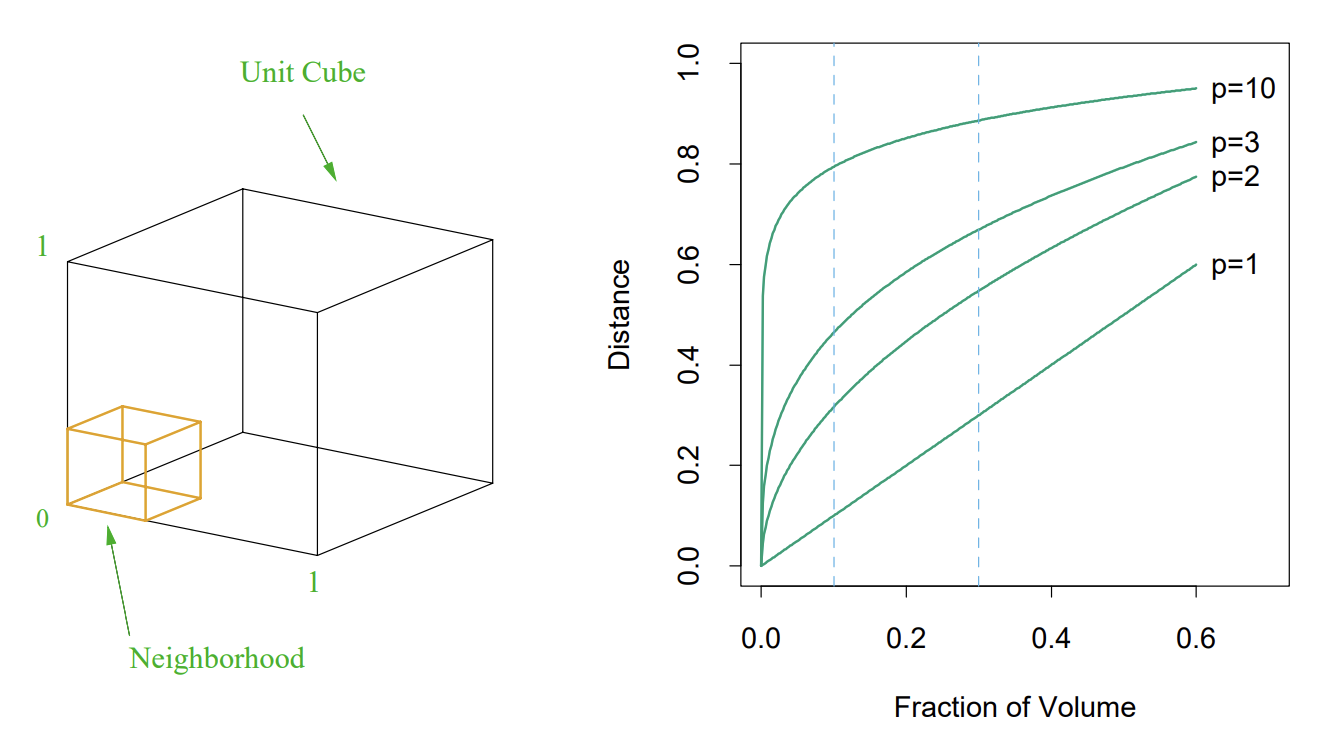
\includegraphics[width=0.8\textwidth]{figures/image.png}
    \caption{Illustration of the curse of dimensionality. Reproduced from \cite{hastie2001}.}
    \label{fig:hypercube}
\end{figure}

The number of features determines a \textit{hypothesis space}, the set of all functions a learning algorithm can choose to map inputs to outputs, and this space grows exponentially as the number of features increases \cite{mitchell1997, goodfellow2016}.

For instance, with $n$ binary features and a binary class, the size of the hypothesis space is $2^{2^n}$. For non-binary features, the size of the hypothesis space grows even more rapidly. For instance, if each feature can take $m$ values and the class has $l$ possible labels, the hypothesis space size becomes $l^{m^n}$, which further emphasizes the importance of feature selection.

\textcolor{red}{ Hypothesis space of a linear regression }


For a fixed-size training dataset, reducing the number of features effectively reduces the number of required training instances. For example, if the number of binary features is reduced from $n = 10$ to $n = 5$, and the total number of training instances $m$ is kept same, the ratio of training instances to possible input combinations, $m / 2^n$, increases exponentially, effectively increasing the coverage of the input space \cite{liu2007}. 

It was demonstrated by Liu and Motoda \cite{liu2007}, feature selection can significantly reduce the hypothesis space by eliminating irrelevant and redundant features, and a smaller hypothesis space makes it easier to identify plausible hypotheses. 

\textcolor{orange}{Removal of the noise}

\textcolor{red}{\cite{blum1997} Definition of relevant and irrelevant features}


Feature selection is process of selecting the most relevant features. Key aspects of feature selection include the selection criterion of the method, evaluation approach, and in some cases search strategy (mainly wrapper methods), \textcolor{green}{ which are discussed in Section XXX}. Based on the selection criterion, most of the feature selection methods belong to one of these \footnote{\textcolor{yellow}{Some methods may not fit into these three categoreies.}}three categories:

\begin{enumerate}
    \item \textbf{Filter methods}: These methods perform feature selection independently of any predictive model. They rely on intrinsic properties of the features, such as correlation, $\chi^2$ tests, or ANOVA \textcolor{pink}{GLOSSARY} to rank the features. Their main advantage is computational speed; however, they do not account for more complex interactions between features, such as non-linear or higher-order dependencies, that might influence the target variable. \textcolor{green}{Section XXs}
    \item \textbf{Wrapper methods}: These methods are a category of feature selection techniques that evaluate subsets of features by training a machine learning model and measuring its performance. They treat the model as a black box and use it to find the combination of features that leads to the best prediction performance. Their main drawback is high computational demand, since the model must be trained multiple times for different feature subsets. \textcolor{green}{Section XXs}
    \textcolor{pink}{GLOSSARY}
    \item \textbf{Embedded methods}: In these methods, feature selection is integrated directly into the model training process. Examples include regularized linear models (e.g., LASSO or Ridge) \textcolor{pink}{GLOSSARY} and tree-based models that provide measures of \textit{feature importance} such as the \textit{Gini coefficient} or \textit{entropy}. \textcolor{green}{Reference to book or chapter}) 
\end{enumerate}


\textcolor{orange}{feaute selection improves interpretability and significantly reduce training time..}

\section{Generalization in Deep Neural Networks}
\label{sec:generalization-neural-networks}

% Deep learning - page 125
For deep neural networks, the hypothesis space is typically extremely large due to to the multiple layers and non-linear activation functions \cite{goodfellow2016}.  


For example, consider the task of recognizing handwritten digits from the MNIST dataset, which contains $70,000$ grayscale images of digits $0$--$9$, and with image dimension of $28 \times 28$ \cite{lecun1998, mnistdataset}.  

A fully connected neural network with one hidden layer of 128 neurons can be used for this task. The hypothesis space - the set of all functions the network can represent - is determined by its parameters. With 784 input neurons, 128 hidden neurons, and 10 output neurons, the network has 

\[
\underbrace{784 \times 128}_{\text{input-to-hidden weights}} + 
\underbrace{128}_{\text{hidden biases}} + 
\underbrace{128 \times 10}_{\text{hidden-to-output weights}} + 
\underbrace{10}_{\text{output biases}} \approx 100{,}000 \text{ parameters.}
\]



Each combination of these values defines a distinct hypothesis, illustrating that even a relatively simple architecture can have a large expressive \textit{capacity}, which is its ability to represent a wide range of functions or patterns in the data.

\textcolor{orange}{Mention XOR problem}



However, such a large hypothesis space can lead to poor generalization. \textit{Generalization} is the ability of a model to perform well on new, unseen data, not just on the data it was trained on. It reflects how well the model captures the underlying patterns rather than memorizing noise.


When the model fits the training data too poorly it said to underfit. \textit{Underfitting} occurs when the chosen hypothesis is too simple relative to the data distribution; this prevents the model from capturing essential patterns and leads to high \textit{training error}.
\textcolor{red}{Training error definition, formula}

\textcolor{orange}{Figure ilustrating Overfitting and underfitting}

Conversely, when the model captures not only essential patterns, but also noise, it is said to overfit. \textit{Overfitting} arises when the hypothesis is more complex than the data on which the model was trained and can lead to high \textit{generalization error}, or also called \textit{test error}.
\textcolor{red}{Establish noise and test error}


To evaluate generalization, the available data is typically divided into separate subsets. The training set is used to fit the model and adjust its parameters, while the test set (or validation set) is kept aside to estimate the model’s performance on unseen data. Measuring the error on the test set provides an estimate of the generalization error, helping to identify underfitting or overfitting of the model.
\textcolor{red}{Training seet, Validation set, test set in more detail}

\textcolor{red}{Give illustative example of underfitting and overfitting}

\textcolor{red}{Add figure-graph showing relation of training and generalization error withregard to number of features}

\textcolor{orange}{Deep learning - page 145}

Important concept tightly linked to overfitting and underfitting is the \emph{bias-variance trade-off}. Let 
\(\hat f(x)\) denote the estimator learned from data, and let \(f(x)\) be the true underlying function we are estimating. The expected prediction error at a point \(x\) can be decomposed as
\[
\mathbb{E}\big[(\hat f(x) - f(x))^2\big]
=
\underbrace{\big(\mathbb{E}[\hat f(x)] - f(x)\big)^2}_{\text{bias}^2}
+
\underbrace{\mathbb{E}\big[(\hat f(x) - \mathbb{E}[\hat f(x)])^2\big]}_{\text{variance}}
+
\sigma^2,
\]
where \(\sigma^2\) is the irreducible noise in the data.

The bias term quantifies the error due to restrictive assumptions in the model. A model with high bias fails to approximate complex patterns and tends to underfit.

The variance, which underlies the problem of overfitting, increases with model complexity. As complexity grows, bias decreases while variance rises. A larger number of parameters allows the model to capture more complex relationships between predictors and the response.

Neural networks, because of their high \emph{capacity} and extremely large hypothesis space, can achieve low bias but often exhibit large variance, especially when the number of parameters is high relative to the sample size. 

For this reason, the goal in practice is to find an appropriate balance:
\[
\text{Generalization Error} \approx \text{Bias}^2 + \text{Variance} + \sigma^2.
\]

Achieving this balance typically requires the use of \emph{regularization techniques}, which will be discussed in \textcolor{green}{subsection X\_x}. For a model with parameters \(\theta\), weight decay (also known as \(L_2\)-regularization) adds a penalty \(\lambda \lVert \theta \rVert_2^2\) to the loss function, and thus effectively reducing variance:
\[
L_{\mathrm{reg}}(\theta) = L(\theta) + \lambda \lVert \theta \rVert_2^2.
\]

Similarly, methods such as dropout, early stopping, and cross-validation help constrain model complexity without sacrificing too much expressive power. These strategies collectively aim to minimize expected test error by controlling variance while keeping bias acceptably low.



\subsection{architerctures, crossvalidation, python pipeline, grid-search, hyperparameters}
\textcolor{orange}{DIVIDING  DATA  INTO  3  CATEGORIES}


